\documentclass[]{scrartcl}

%Packages________________
\usepackage[normalem]{ulem}
\usepackage{cancel, xcolor}
\usepackage{parskip}
\usepackage{caption, subcaption}
\usepackage[Spanish,es-tabla,es-noshorthands]{babel}
\usepackage{newtxtext}
\usepackage[varvw]{newtxmath}
\usepackage{booktabs, colortbl, bigstrut, multirow, multicol}
\usepackage{url}
\usepackage{pgfplots}
\usepackage{graphicx}
\usepackage{amsmath}
\usepackage{tabularx}
\usepackage{floatrow}
\usepackage{float}
\usepackage{cancel}
\usepackage[spanish]{cleveref}
\usepackage{tikz}
\usetikzlibrary{arrows.meta}
\crefname{table}{tabla}{tablas}
\usepackage{wrapfig}
\usepackage{adjustbox}
\usepackage{geometry}
\usepackage{lipsum}
\usepackage{fancybox}
\geometry{
	top=2.4cm,
	bottom=2.4cm,
	left=2.3cm,
	right=2.3cm
}

\usepackage[
    backend=biber,
	citestyle=verbose-ibid,
    bibstyle=authoryear-icomp,
    natbib=true,
    url=true, 
    doi=true,
    eprint=false
]{biblatex}

\addbibresource{ref.bib}

%Commands________________
\newcommand\hcancel[2][black]{\setbox0=\hbox{$#2$}%strikeout
\rlap{\raisebox{.45\ht0}{\textcolor{#1}{\rule{\wd0}{1pt}}}}#2} 

\renewcommand\theequation{\Alph{equation}}

\DeclareMathOperator\Log{Log}
\DeclareMathOperator\Ln{Ln}


%\renewcommand\thesubsection{\Alph{subsection}}

%Titlepage_________________
\title{\vspace{-1.8cm} Práctica de Simulación 3 - Bloque 1}
\author{Álvaro Jerónimo Sánchez}
\date{08/03/2026}

%Document_____________
\begin{document}
\maketitle
\setcounter{section}{0}
\renewcommand{\tablename}{Tabla}

\section{Práctica 3:}

\subsection{Ejercicio 1}

\begin{figure}[h]
\centering
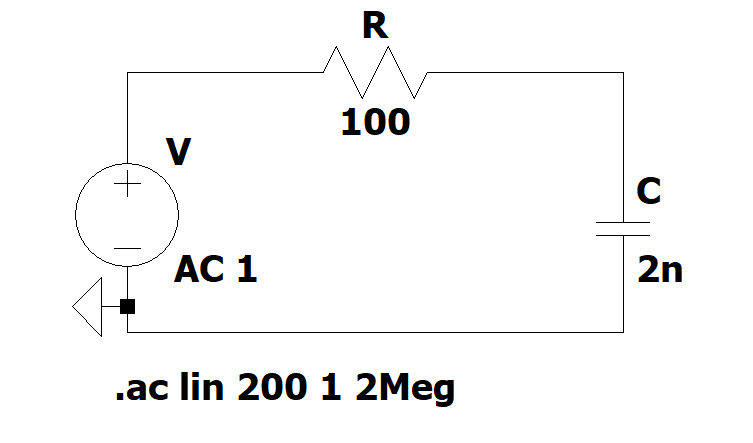
\includegraphics[width=0.5\columnwidth]{../3-1.png}
\end{figure}

\begin{wrapfigure}{r}{0.5\textwidth}
\centering
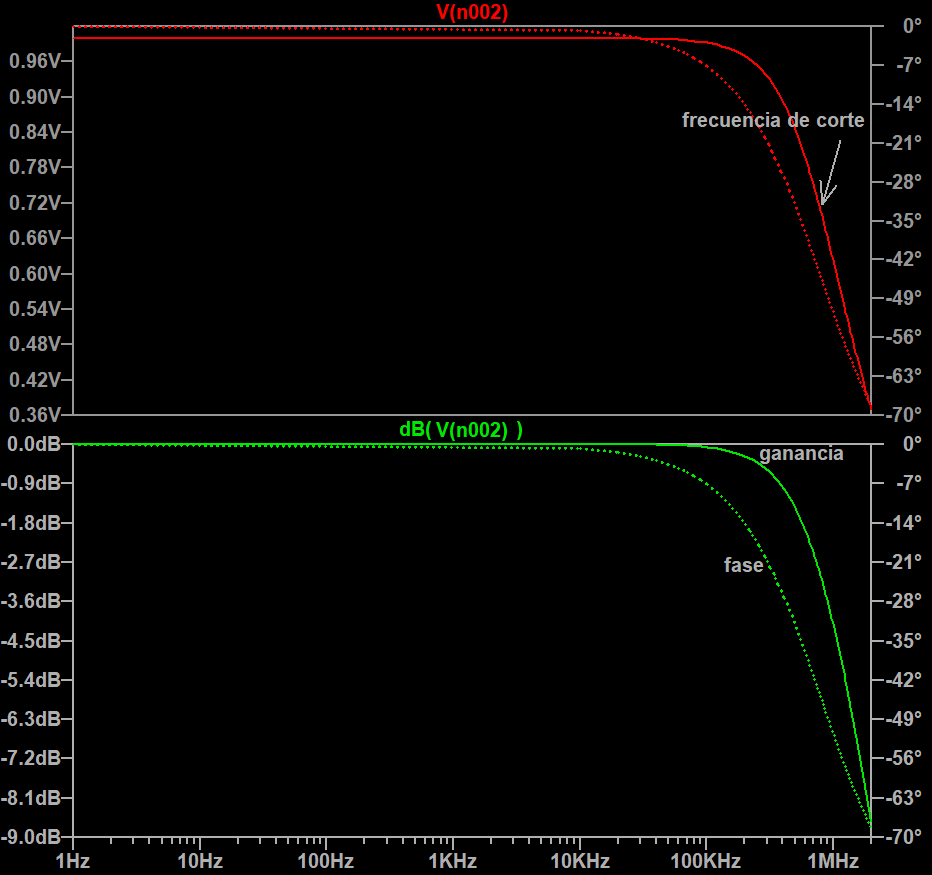
\includegraphics[width=0.95\columnwidth]{../3-1g.png}
\end{wrapfigure}

Para este circuito se ha tenido que realizar un barrido de corriente alterna, que modula la frecuencia de la misma de un valor a otro escogido y devuelve los resultados del circuito para cada frecuencia. Se ha usado un barrido lineal, para poder elegir el orden de los incrementos. Para tener un barrido con incrementos de $10\, kHz$, debemos indicar que queremos que tenga $200$ puntos, ya que $\frac{2000000-1}{10000}\approxeq 200$. Observamos que para frecuencias altas, la ganancia en decibelios es $0$, y al ser una escala logarítmica, significa que $\frac{V_{out}}{V_{in}}=1$, valor que esperamos ya que el filtro \textbf{pasa-baja} permite el paso de las frecuencias más bajas. En cambio, observamos que conforme la frecuencia va aumentando, la ganancia se vuelve más negativa, es decir, que $\frac{V_{out}}{V_{in}}$ es decimal, por lo que está siendo atenuado.

En la gráfica de $V(n002)\, / \, f$, la frecuencia de corte será aquella en la que $V_{out}=0.707V_{in}$. En este caso, como se ha elegido amplitud inicial de $1\, V$, será justo en $0.707\, V$. Gráficamente nos da un valor de frecuencia de aproximadamente $800\, Hz$, que coincide con el valor teórico calculado: $f_c=\frac{1}{2\pi RC}=795.77\, Hz$.

\clearpage

\subsection{Ejercicio 2}

\begin{figure}[h]
\centering
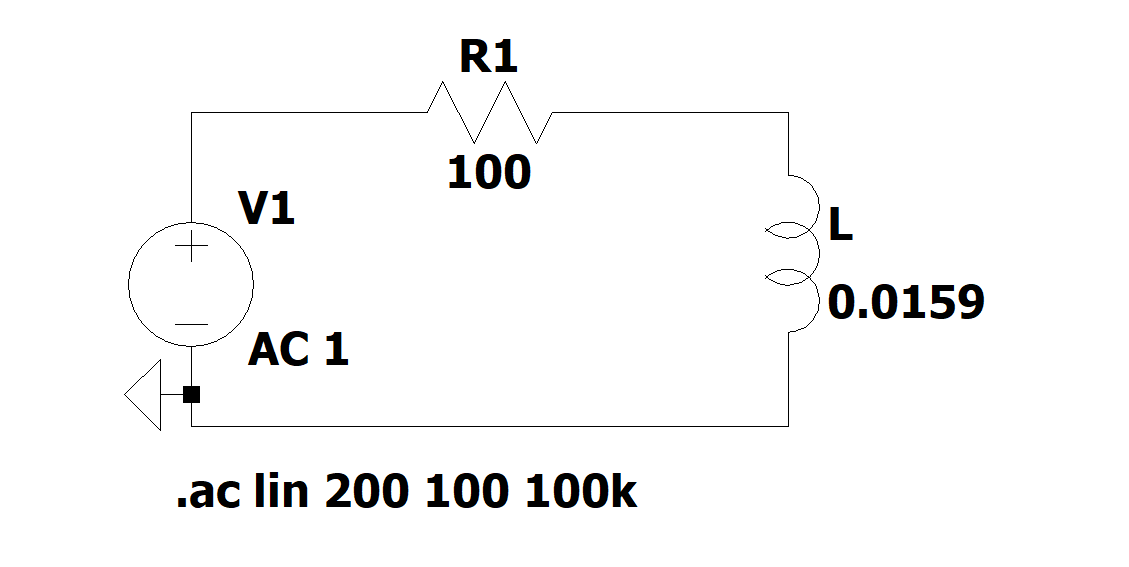
\includegraphics[width=0.6\columnwidth]{../3-2.png}
\end{figure}

\begin{wrapfigure}[10]{r}{0.5\textwidth}
\centering
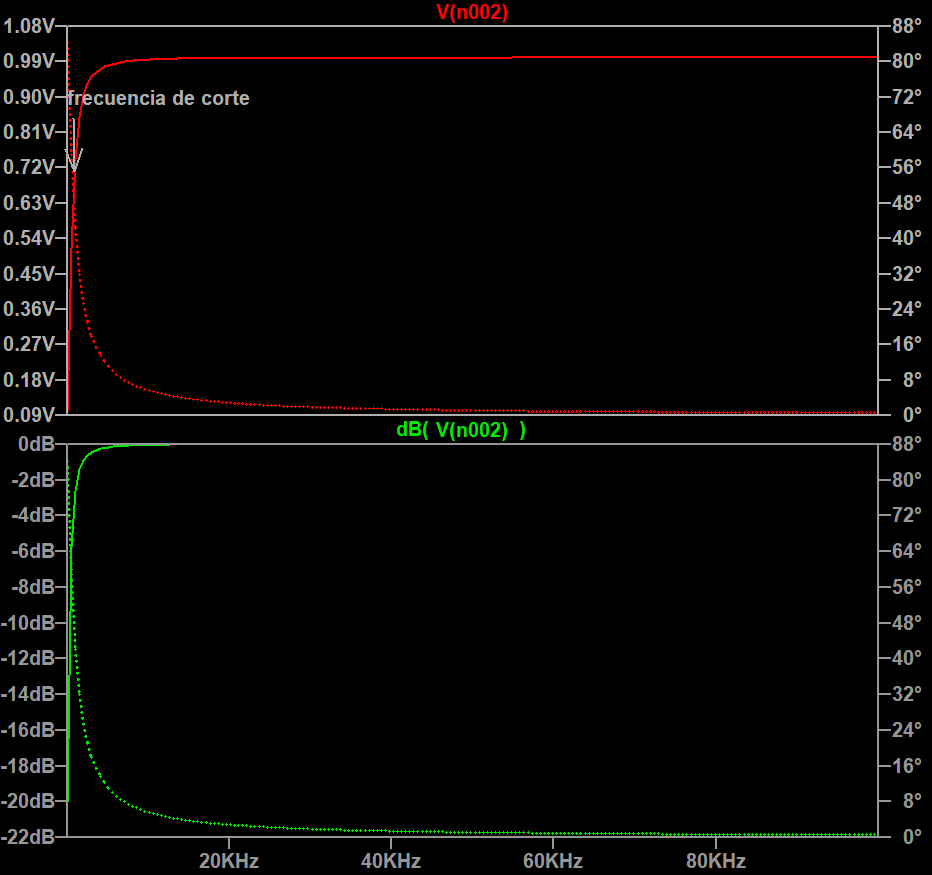
\includegraphics[width=0.95\columnwidth]{../3-2g.png}
\end{wrapfigure}

Se ha pedido que para este ejercicio la frecuencia de corte del filtro sea $f_c=\frac{R}{2\pi L}=1000\, Hz \Rightarrow L=0.0159\, H$. Tras realizar el barrido con este dato introducido, hallamos gráficamente que la frecuencia de corte es aproximadamente $1.029\, kHz$, resultado que cuadra con el enunciado del ejercicio.

Se ha realizado también el diagrama de Bode (en $dB$), representado con una traza verde, al igual que en el ejercicio anterior. 

\vspace{2.8cm}
\subsection{Ejercicio 3}

\begin{wrapfigure}[10]{r}{0.5\textwidth}
\centering
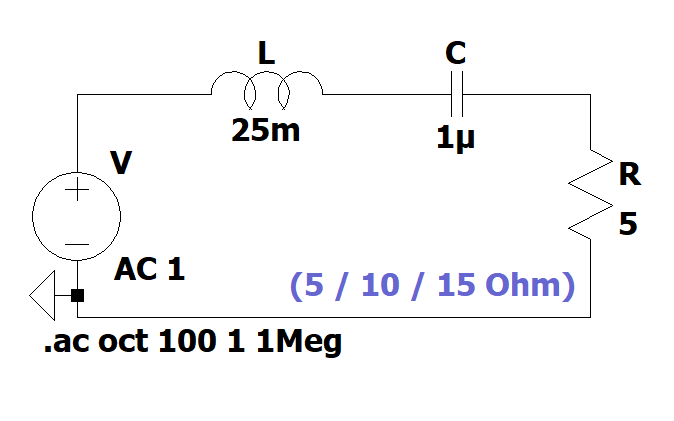
\includegraphics[width=0.95\columnwidth]{../3-3.png}
\end{wrapfigure}

Para este circuito nos piden hacer tres barridos cambiando la resistencia a $5\, \Omega,\, 50\, \Omega\, \text{ y } 100\, \Omega$. Se pueden hallar los valores teóricos de la anchura de banda, definida por: $\Delta f =f_2-f_1$, siendo éstas las frecuencias de corte correspondientes a las atenuaciones realizadas por el condensador y la bobina. Conociendo que el factor Q de un cirucito \textit{RLC} es $Q=\frac{f_o}{\Delta f}$, y sabiendo que la frecuencia de resonancia está determinada por $f_o=\frac{1}{2\pi\sqrt{LC}}$, sustituimos y despejamos:

%graphs


\begin{minipage}{.4\textwidth}
	\begin{gather*}
	f_o=\frac{1}{2\pi\sqrt{LC}} = 1006.5\, Hz\\
	Q=\frac{1}{R}\sqrt{\frac{L}{C}}\; ; \; \Delta f = \frac{f_o}{Q}
\end{gather*}
\end{minipage}
\hfill\vline\hfill
\begin{minipage}{.4\textwidth}
	\begin{table}[H]
\centering
%\def\arraystretch{1.5}
\begin{tabular}{|c||c|c|} \cline{2-3}
	\multicolumn{1}{c|}{} & \textbf{Q} & \textbf{$\Delta f$} \\ \hline
	$5\, \Omega$ & $31.62$ & $31.83\, Hz$ \\ \hline
	 $10\, \Omega$ & $15.81$ & $63.66\, Hz$ \\ \hline
	$15\, \Omega$  & $10.54$ & $95.49\, Hz$ \\ \hline
\end{tabular}
\end{table}
\vspace{2pt}
\end{minipage}
\hrule

\clearpage

\begin{wrapfigure}{r}{0.4\textwidth}
\centering
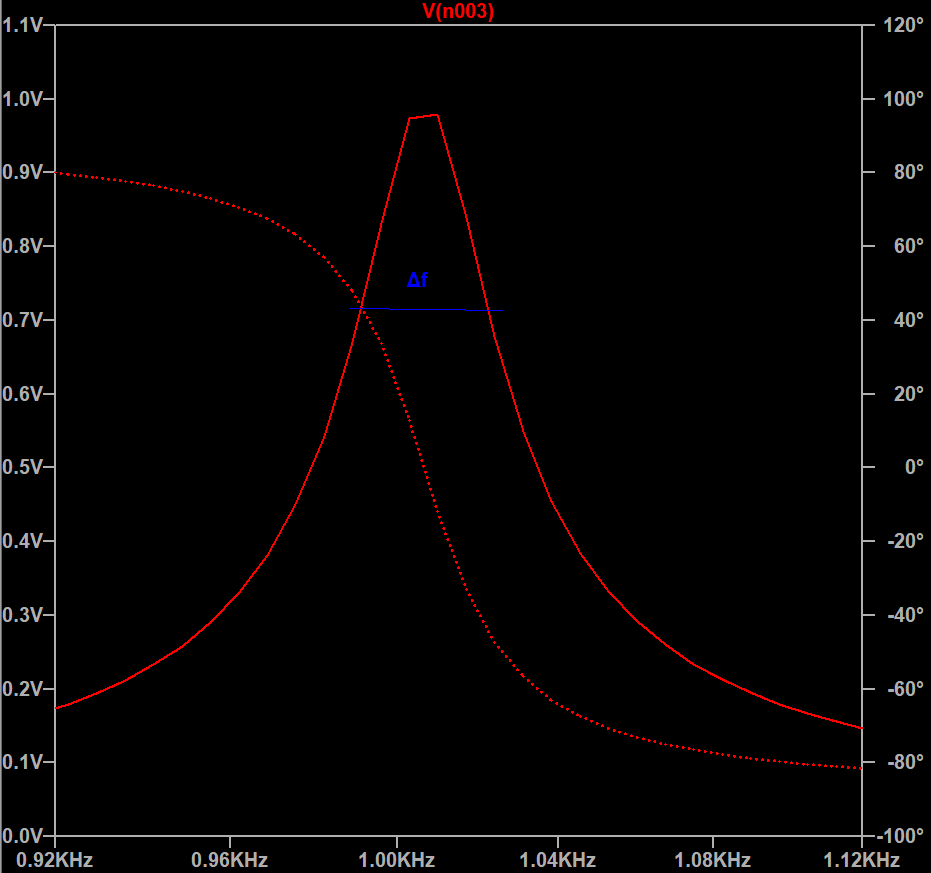
\includegraphics[width=0.95\columnwidth]{../3-med.png}
\end{wrapfigure}

Comparando los resultados teóricos con los hallados gráficamente, podemos observar que la frecuencia de resonancia coincide, siendo esta $\approx 1 kHz$. El ancho de banda lo medimos con la diferencia de las dos frecuencias de corte (en $V\approx 0.707\, V$) correspondientes a las atenuaciones por cada lado, y en todos los casos también coinciden con los teóricos. Ha sido necesario hacer zoom en la gráfica para poder apreciarlo, como se indica en el ejemplo de la derecha.

A continuación se muestran las gráficas para cada resistencia ordenadas por columnas. Dentro de cada columna, la traza roja representa el voltage frente a la frecuencia, mientras que la verde es el diagrama de Bode (\textit{hacer zoom en el PDF para ver con mayor resolución}):

\begin{figure}[h!]
	\centering
	\begin{minipage}{.32\textwidth}
	  \centering
	  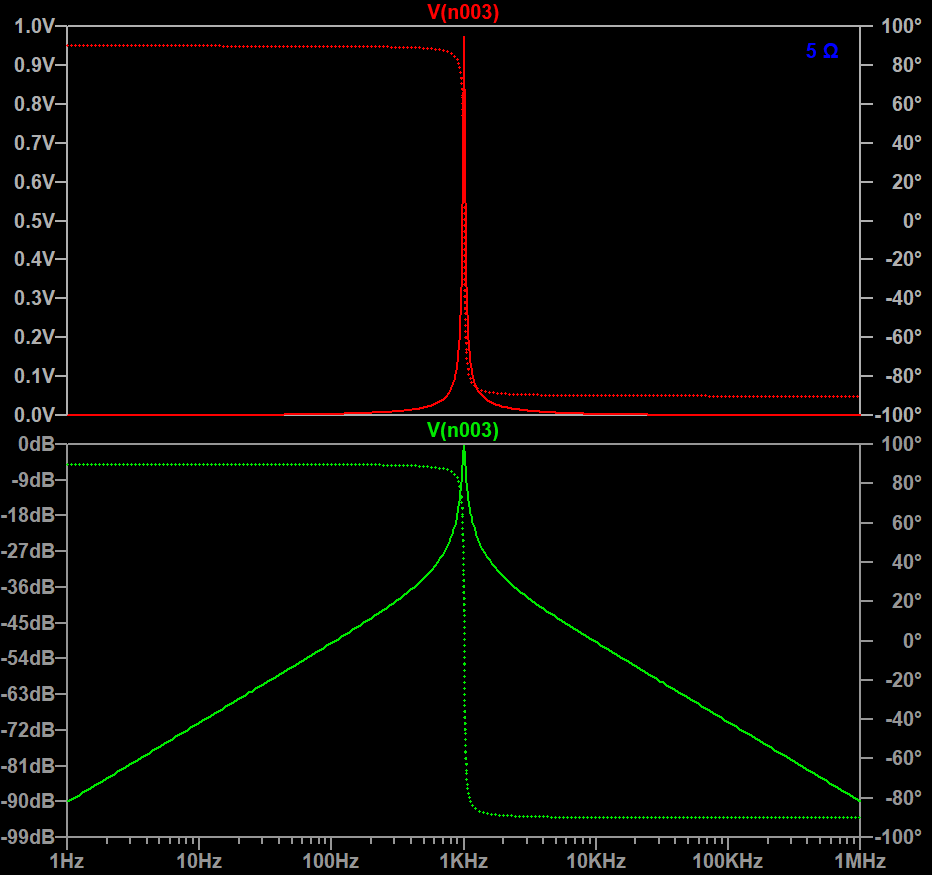
\includegraphics[width=\linewidth]{../3-35.png}
	\end{minipage}
	\begin{minipage}{.32\textwidth}
	  \centering
	  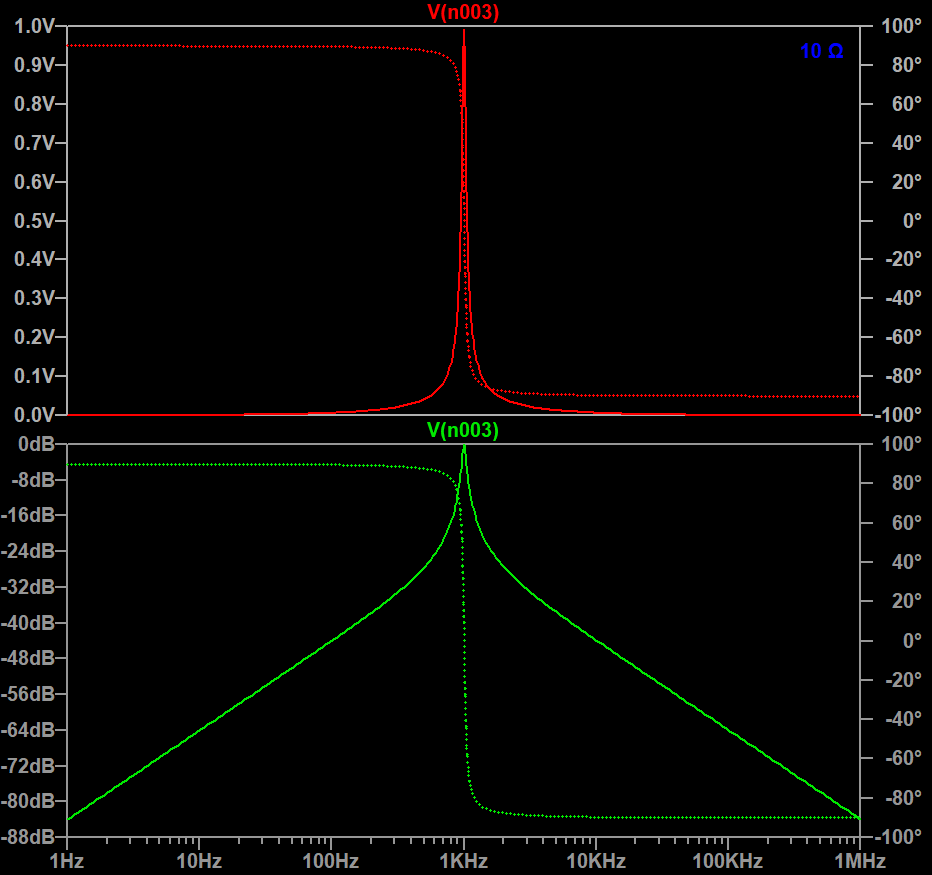
\includegraphics[width=\linewidth]{../3-310.png}
	\end{minipage}
	\begin{minipage}{.32\textwidth}
	  \centering
	  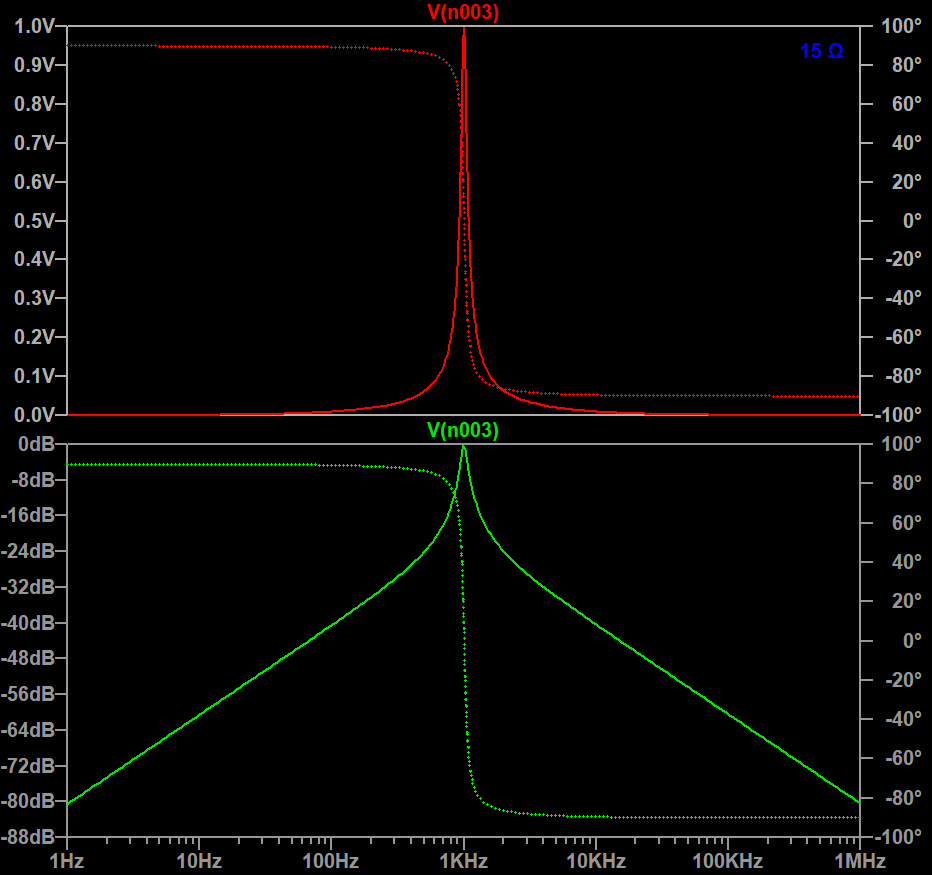
\includegraphics[width=\linewidth]{../3-315.png}
	\end{minipage}
	\end{figure}

% _________________________________________

\vspace{2cm}
\begin{center}
\setlength{\fboxsep}{0.5cm}
\shadowbox{\begin{minipage}{10.5cm}
\textbf{Declaración de Autoría}\\

El alumno
Álvaro Jerónimo Sánchez
, con DNI número 
09847051S
, declara que es el autor único e individual de este trabajo.\\

\vspace{3cm}
Fdo:

\end{minipage}}
\end{center}

\end{document}